\documentclass[border=10pt]{standalone}

\usepackage{tikz}
\usepackage{tikzsymbols}
\usetikzlibrary{calc,patterns,shapes.geometric}

\def\centerarc[#1](#2)(#3:#4:#5){\draw[#1] ($(#2)+({#5*cos(#3)},{#5*sin(#3)})$) arc (#3:#4:#5);}

\begin{document}
	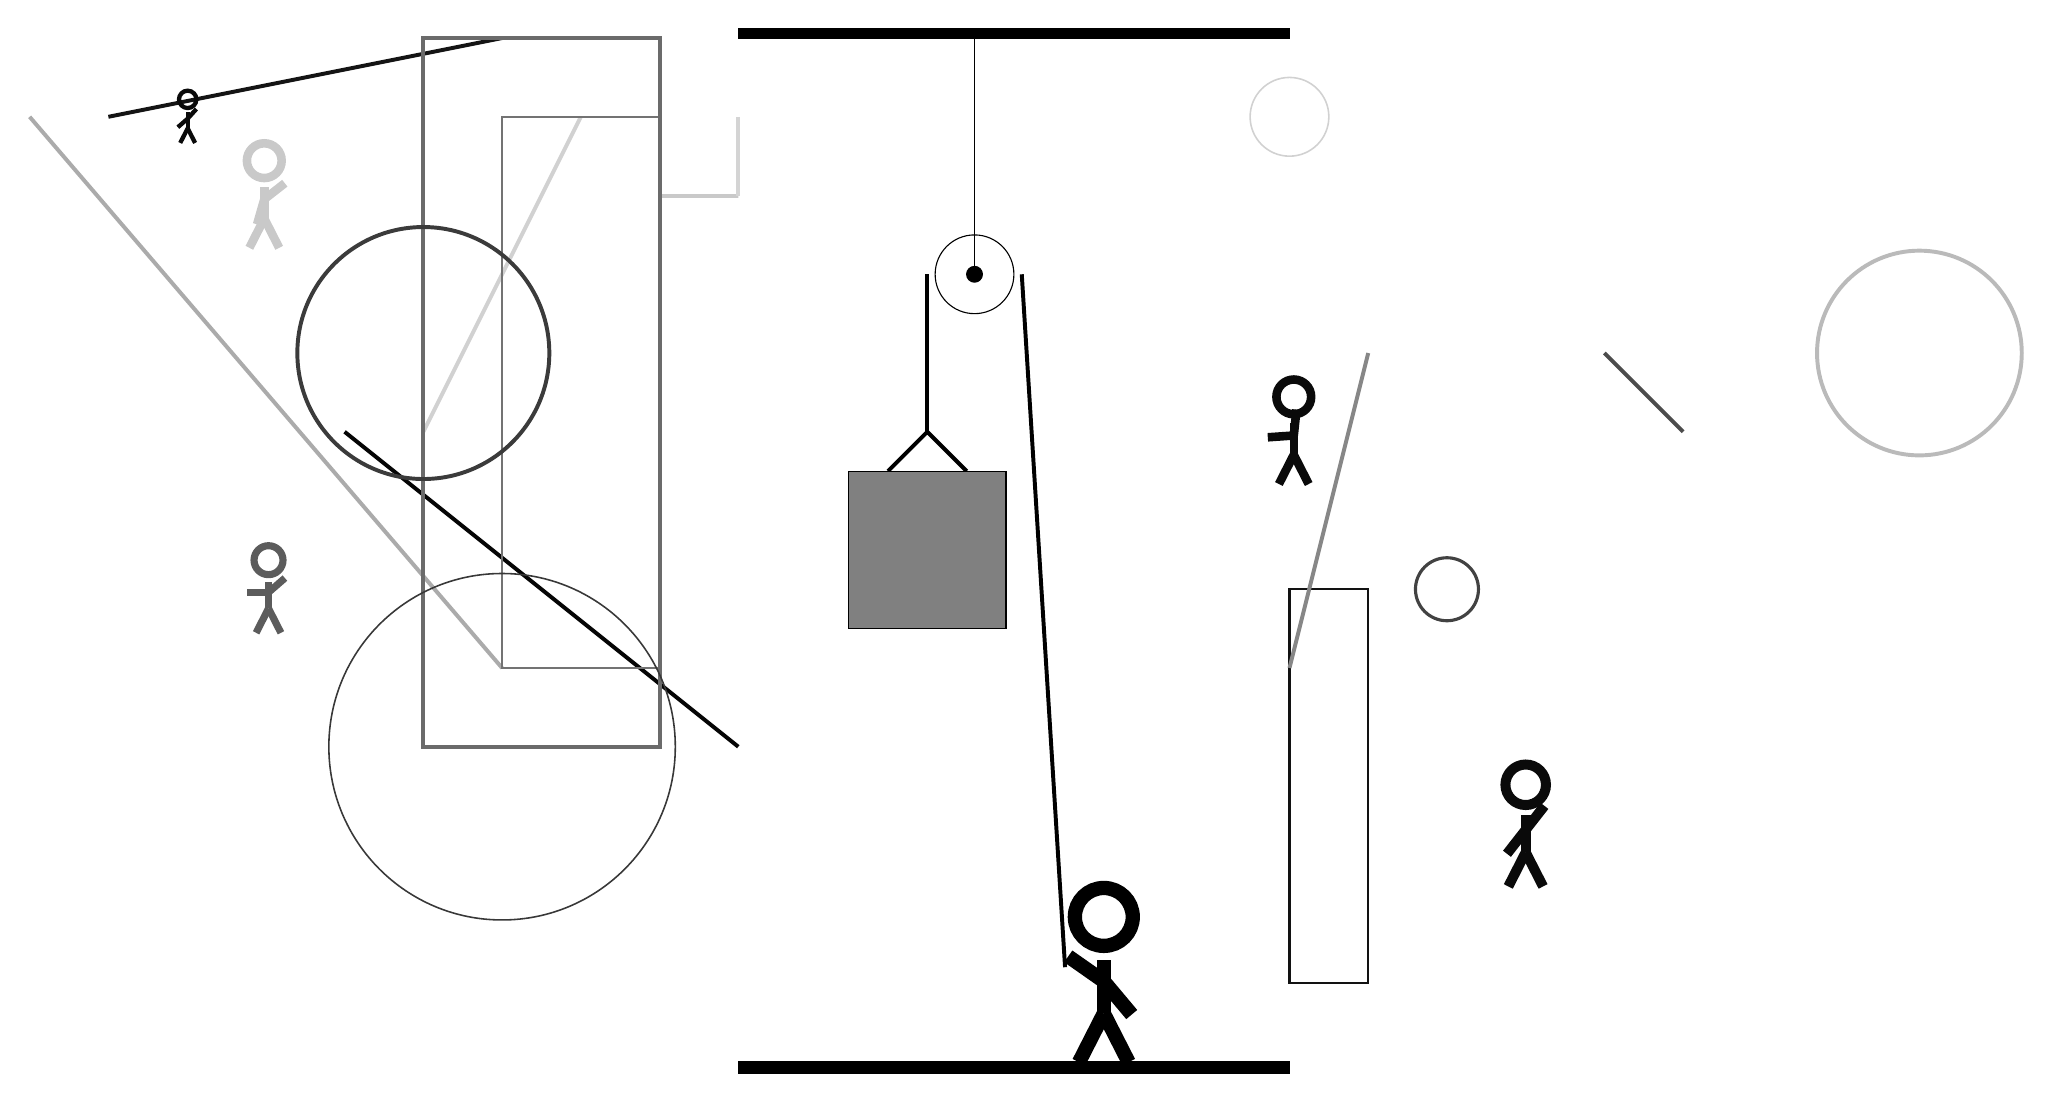
\begin{tikzpicture}
		%%%%% START %%%%%
		
		\draw[fill=black] (-2, 10) rectangle (5, 10.125);
		
		\draw (1, 7) circle (0.5);
		\draw[fill=black] (1, 7) circle (0.1);
		\draw (1, 10) -- (1, 7);
		
		\draw[line width=0.5mm] (-0.1, 4.5) -- (0.4, 5.0) -- (0.9, 4.5);
		\draw[fill=black!50] (-0.6, 4.5) rectangle (1.4, 2.5);
		
		\draw[line width=0.5mm] (0.4, 7) -- (0.4, 5.0);
		\centerarc[line width=0.5mm](1, 7)(0:180:0.6);
		\draw[line width=0.5mm](1.6, 7) -- (2.15, -1.8);
		
		\draw[line width=0.5mm, color=black!98](-2, 1) -- (-7, 5);
		
		\draw [line width=0.2mm, color=black!18](5, 9) circle (0.5);
		\draw[line width=0.3mm, color=black!93] (5, 3) rectangle (6, -2);
		\draw[line width=0.5mm, color=black!33](-5, 2) -- (-11, 9);
		\draw[line width=0.5mm, color=black!47](6, 6) -- (5, 2);
		
		\draw[line width=0.5mm, color=black!21] (-3, 8) rectangle (-2, 8);
		\draw [line width=0.5mm, color=black!27](13, 6) circle (1.3);
		\draw[line width=0.5mm, color=black!92](-5, 10) -- (-10, 9);
		\node[line width=0.2mm, color=black!64] at (-8, 3) {\Strichmaxerl[5][0][41]};
		
		\draw[line width=0.5mm, color=black!18](-6, 5) -- (-4, 9);
		\draw [line width=0.4mm, color=black!74](7, 3) circle (0.4);
		\draw[line width=0.3mm, color=black!55] (-3, 9) rectangle (-5, 2);
		\node[line width=0.5mm, color=black!96] at (-9, 9) {\Strichmaxerl[3][41][48]};
		
		\draw[line width=0.5mm, color=black!70](9, 6) -- (10, 5);
		\node[line width=0.6mm, color=black!96] at (5, 5) {\Strichmaxerl[6][4][84]};
		\node[line width=0.4mm, color=black!96] at (8, 0) {\Strichmaxerl[7][52][52]};
		\node[line width=0.7mm, color=black!21] at (-8, 8) {\Strichmaxerl[6][74][38]};
		\draw[line width=0.5mm, color=black!58] (-3, 10) rectangle (-6, 1);
		\draw [line width=0.5mm, color=black!77](-6, 6) circle (1.6);
		\draw[line width=0.5mm, color=black!17](-2, 9) -- (-2, 8);
		\draw [line width=0.2mm, color=black!78](-5, 1) circle (2.2);
		
		
		\node at (2.6, -1.9) {\Strichmaxerl[10][-35][-50]};
		
		\draw[fill=black] (-2, -3) rectangle (5, -3.15);
		
		%%%%% END %%%%%
	\end{tikzpicture}
\end{document}